\documentclass[12pt]{article}
\usepackage[utf8]{inputenc}
\usepackage[T1]{fontenc}
\usepackage{graphicx}
\graphicspath{ {./images/} }
\usepackage{xcolor}

%%novalidate

\usepackage{tikz}
\usepackage{calc}
\usepackage{booktabs}
%\usepackage{hyperref}

% colors
\definecolor{color1}{HTML}{333333}
%\definecolor{color1}{HTML}{8C260F}
\definecolor{color2}{HTML}{333333}


% fonts
\usepackage{fontspec}
\defaultfontfeatures{Mapping=tex-text}
\setmainfont
[BoldFont=FiraCode-Bold.ttf,
ItalicFont=Lato-Italic.ttf,
BoldItalicFont=Lato-BoldItalic.ttf]
{Lato-Regular.ttf}
\newfontfamily\headingfont[ItalicFont=Lato-BlackItalic.ttf]{FiraCode-Bold.ttf}
%%%

\usepackage{geometry}
\geometry{a4paper,
hmargin=20mm,vmargin=20mm,
head=0ex,foot=3ex}

\linespread{1.3}

\usepackage[hang]{caption}
\DeclareCaptionFormat{upper}{#1#2\uppercase{#3}\par}
\captionsetup{labelfont={bf,color=color2},textfont={normalsize,color=color2},format = upper,figurename=FIGURE,tablename=TABLE}

%%% fancy sections
\usepackage{titlesec}
%\titleformat{\chapter}{\headingfont\LARGE\bfseries\scshape\color{color1}}{\thechapter}{1em}{}[\titlerule]
\titleformat{\section}{\color{color1}\headingfont\Large\bfseries\uppercase}{\thesection}{1em}{}[\titlerule]
\titleformat{\subsection}{\color{color1}\headingfont\large\bfseries\uppercase}{\thesubsection}{1em}{}
\titleformat{\subsubsection}{\color{color1}\headingfont\bfseries\uppercase}{\thesubsubsection}{1em}{}
%%%

% head and foot
\usepackage{fancyhdr}
\pagestyle{fancy}
\lhead{}
\chead{}
\makeatletter
\rhead{\color{color2}\@date}
\makeatother
\newlength{\myheight}
\lfoot{
\settoheight{\myheight}{\thepage}
\raisebox{-2ex-0.5\myheight}{
\includegraphics[height=4ex]{logo}}
}
\cfoot{\color{color2}Noisebridge Case Statement}
\rfoot{\color{color2}\thepage}
\renewcommand\headrulewidth{0pt}
\renewcommand\footrulewidth{0pt}

%%% picture on cover page
\usepackage{eso-pic}
\newcommand\BackgroundPic{%
\put(0,0){%
\parbox[b][\paperheight]{\paperwidth}{%
\vfill
\centering

\includegraphics[width=\paperwidth,height=\paperheight,%
keepaspectratio]{cover}%
\vfill
}}}
%%%
% custom titlepage
\makeatletter
\renewcommand{\maketitle}{
\thispagestyle{empty}
\AddToShipoutPicture*{\BackgroundPic}
\ClearShipoutPicture
%
\phantom{a}
\vfill
\phantom{a}\hfill
\begin{tabular}[c]{@{}p{0.7\textwidth}@{}}
      \color{white}\headingfont\LARGE\@title\\[1em]
      \color{white}\headingfont\Large\@author\\[2em]
\end{tabular}
%
\clearpage
}
\makeatother
%%%


%%% fancy boxes
\usepackage{tcolorbox}
\usepackage{wrapfig}
\def\fullboxbegin{
\bigskip
\begin{tcolorbox}[colback=color1,colframe=color1,coltext=white,arc=0mm,boxrule=0pt]
}
\def\fullboxend{\end{tcolorbox}\medskip}
%
\def\leftboxbegin{
\begin{wrapfigure}{l}{0.5\textwidth}
\begin{tcolorbox}[colback=color1,colframe=color1,coltext=white,arc=0mm,boxrule=0pt]
}
\def\leftboxend{
\end{tcolorbox}
\end{wrapfigure}
}
%
\def\rightboxbegin{
\begin{wrapfigure}{r}{0.5\textwidth}
\begin{tcolorbox}[colback=color1,colframe=color1,coltext=white,arc=0mm,boxrule=0pt]
}
\def\rightboxend{
\end{tcolorbox}
\end{wrapfigure}
}
%
\newcounter{frames}
\def\frameboxbegin#1{
\bigskip
\refstepcounter{frames}
\begin{tcolorbox}[colback=white,colframe=color1,arc=0mm,title={\MakeUppercase{\textbf{Frame \arabic{frames}}: #1}}]
}
\def\frameboxend{
\end{tcolorbox}
}
%%%

\usepackage{lipsum}

%%%%%%%%%%%%%%%
% Title Page
\title{Noisebridge Case Statement}
\author{Fundraising Working Group \newline Noisebridge \newline 2169 Mission St., 3rd floor \newline San Francisco, CA 94110}
\date{\today}
%%%%%%%%%%%%%%%

\begin{document}
\maketitle

\tableofcontents
\clearpage

\section{Organization Info}

\subsection{Mission}

Noisebridge is a safe and welcoming environment providing resources that enable anyone to learn, create, and hack. Noisebridge is funded by donations and evolves by engagement from the whole community. We enable a wide variety of community activities, from electronics hacking to sewing to wood and metal working, from 3D printing to 3D modeling and VR development.

\subsection{History and Impact}

Noisebridge began in 2007 as an idea in the minds of a few excited hackers at the 24th Chaos Communication Congress, taking inspiration from cbase in Berlin and Metalab in Vienna. The first physical location for Noisebridge, in the Mission district of San Francisco, was acquired in 2008, and within a few short months, the packed 1000-or-so square foot space was getting cramped. Noisebridge acquired its current space just a few blocks away from the previous one. In 2014 we had a major reboot of the current space, which significantly refurbished infrastructure, and in 2016 we undertook the construction of a combined metalshop and lasercutter workshop.

Numerous significant projects have had roots at Noisebridge over the years:

\vspace{0.5em}

\begin{itemize}
    \item The Diaspora social network began at Noisebridge
    \item The Pursuance Project — a secure, open source collaboration tool for activists, journalists, and nonprofits — is actively developed by multiple members of the Noisebridge community
    \item 3D printer company Type A machines started at Noisebridge and built their earliest machines here
    \item The Unityversity interactive game development environment is built and maintained by a long time Noisebridge member
\end{itemize}

\vspace{0.5em}

We've also been an influence on contemporary literature and digital culture:

\vspace{0.5em}

\begin{itemize}
    \item Cory Doctorow's novel Homeland features Noisebridge as the home hackerspace of one of its characters
    \item Annalee Newitz wrote parts of the novel Autonomous at Noisebridge
    \item Ubisoft's based the hacker headquarters in Watchdogs 2 on Noisebridge
    \item The Aaron Swartz Museum/Art Gallery VR Installation is developed primarily by members of the Noisebridge community
\end{itemize}

\subsection{Current Events and Programs}

Noisebridge has many classes and meetups. For the last decade, participants at Noisebridge have run a weekly soldering and introductory electronics class called Circuit Hacking Mondays. Along side this class on Mondays, there are regular Python classes, at both an introductory and intermediate level. Tuesdays have a Unity game development and VR class called Gamebridge Unityversity.

Until mid 2017, we also had long running web development classes on Wednesdays. We've also sporadically had classes on Haskell, category theory, type theory, Arduino, introductory sewing, and many other topics.

All of these classes are taught by people who are passionate about the subject matter, and about helping others learn. None of them were paid by Noisebridge, nor by the students: they taught these classes because they believed in sharing knowing and helping others level up their skills.

Noisebridge has also hosted many regular meetups in its history. There are currently a number of groups using Noisebridge to host events, including whiteboarding self-guided group study groups, cryptogovernance enthusiasts, hobby roboticists, Ableton music makers, noise music and video experimentalists, sewing and bag making fabric artists, and cypherpunks who work on new privacy technology. As with everything at Noisebridge, these meetups are run for free, by people who are excited to help the local community and also the world at large.

We also host talks, mini-conferences, and guest lecturers. Every third Thursday is 5 Minutes of Fame, which is an unconference style event where anyone can give a 5 minute talk on any topic of their choosing. We've had talks by world renowned academic computer scientists on topics such as functional programming and cryptography. We've also hosted interviews and gatherings with prominent privacy and security advocates, including Barrett Brown and Chelsea Manning.



\subsection{Finances}

Monthly income has averaged a \$12,000 over the last 6 months, with sources broken down as follows:

TODO

These figures have trended upward over the last TODO years:

Monthly expenses total on average \$10,000, broken down as follows:

\begin{itemize}
    \item Rent: \$6,500
    \item Utilities: \$1,300
        \begin{itemize}
            \item Electricity: \$500
            \item Trash: \$550
            \item Water: \$150
            \item Internet: \$75
        \end{itemize}
    \item Snacks: \$1,600.00
        \begin{itemize}
            \item Club Mate: \$700
            \item Other Snacks: \$900
        \end{itemize}
    \item Administration: \$450
        \begin{itemize}
            \item Accounting: \$250
            \item Insurance: \$200
        \end{itemize}
    \item T-shirts, stickers, etc.: \$200
    \item Misc. \$50
\end{itemize}

These figures have remained fairly stable over the last TODO years, modulo the introduction of new spending categories:

TODO

\section{Organizational Constituency}

In some sense, Noisebridge serves the entire world: we're open to everyone, everywhere. But because of the limitations of physical space, our biggest constituency is in the San Francisco Bay Area. Our educational events have a wide range of attendees: during Circuit Hacking Mondays, for example, it's not uncommon for about half the participants to be children and young adults whose parents support their interests in electronics and technology. Our programming events are typically attended by adults who are working in the tech industry, or interested in learning to program so they can get jobs in the tech industry but who don't have the resources required by a bootcamp. Participants in Noisebridge span a huge range of income levels, as well. A significant fraction are employees at tech companies in Silicon Valley. A number of others are unemployed or homeless, and are able to use Noisebridge to work on things to improve their life, repair clothing, gain new skills, etc.

Precise numbers for participation at Noisebridge are hard to come by. Partly this is because we are open to the public not everyone has RFID access that would enable automatic tracking, and partly this is because we have intentionally avoided tracking people for privacy reasons. There are approximately 200 regular participants in Noisebridge, but the number of people who come here and use the space every few months is much larger, in the range of 1000, possibly more. Noisebridge is also used as a temporary home base for hackers who travel to SF from other parts of the world, and so the total number of people who have benefit from Noisebridge and made use of the space and its resources over the years probably reaches into the tens of thousands.

Activities done at Noisebridge have even greater reach, however. Because we support open source software projects and related technologies, the reach of the Noisebridge community extends to the entirety of the networked world. Numerous social impact projects have started or been run out of Noisebridge, including the Diaspora social network and the Pursuance Project. Many startups and small businesses have been run out of Noisebridge during their early days, including the 3D printer company Type A Machines and Outershell Adventure. Employees at startups often use Noisebridge to hack on prototypes of products, such as the robot delivery company Kiwi Campus.

\section{Organizational Distinctiveness}

Anyone can participate in Noisebridge for free; no membership fees or entrance fees are required to use Noisebridge. Anyone can teach classes or hold meetups in the space free of charge, provided that the events themselves are also open to everyone free of charge. We're entirely funded by donations, and run by the community; no one is in charge of Noisebridge, and everyone is in charge of Noisebridge.

Everything happens at Noisebridge do-ocratically: if someone thinks it should be done, they're empowered to do it. This makes Noisebridge an incredibly dynamic environment, changing in response to needs of the community as soon as they arise. It also provides a glimpse into a whole new world of project and community organizing, as most people have never been in a situation where they can radically alter their surroundings and build whatever they want, without having to ask permission first.

\section{Capital Plans}

Our fundraising goal is to raise between \$1 million and \$4 million from various kinds of donors. We are working with the fundraising consultancy Scandiuzzi Krebs to achieve these goals. We'll be reaching out to tech companies of all sizes because of the deep connections that Noisebridge has to the tech industry, both in serving their employees and also supporting their work. We'll also be reaching out to governmental agencies that promote education, the arts, and innovation. Finally, we'll be inviting individual donors to support Noisebridge, especially visionaries and philanthropists concerned about the future of STEAM education and the democratization of technology.

\section{Vision}

\section{Campaign Team}

\subsection{Ruth Grace Wong}

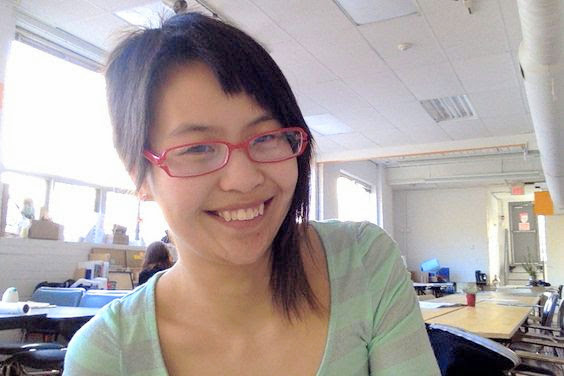
\includegraphics[width=6cm]{ruth}

Ruth is a Site Reliability Engineer at Pinterest by day and a manufacturing engineer by night. She does lots of sewing and laser cutting projects at Noisebridge. The work she does in building her skills and sharing her projects at Noisebridge has lead to many opportunities, such as her Leave Me Alone Sweater collaboration with Betabrand, an acrylic prototyping gig and part time manufacturing job with Aqua Design Innovations, and a writing gig with Supplyframe Hardware.

She can be contacted at her full name at gmail.com.

\subsection{Kevin Prichard}

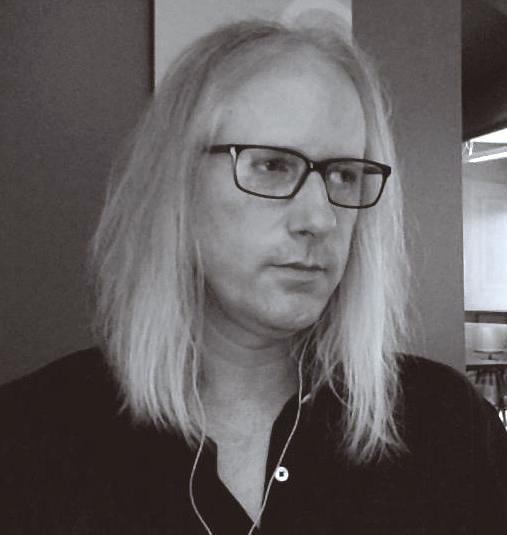
\includegraphics[width=6cm]{Mister_name}

Kevin Prichard volunteers as an electronics instructor at Noisebridge, is a mentor for programmers seeking to improve their job interview skills, and works as a backend software engineer in the travel industry.

\section{Budgets}

\subsection{Constraints on Locations}

Any property that Noisebridge acquires, whether for leasing or purchasing, ought to satisfy the following constraints:

\begin{itemize}
    \item In San Francisco
    \item Close to BART
    \item $\geq$6,000 sf
    \item TODO What zoning PRECISELY?
    \item 100A minimum power supply
    \item Accessible
        \begin{itemize}
            \item ADA bathroom
            \item Elevator access or ground floor
        \end{itemize}
\end{itemize}

\subsection{Cost of Improvement}

Because Noisebridge needs industrial space, very little improvement will take place in any new location we acquire. Removal and construction of internal walls and other infrastructure at the current 2169 Mission St location was done entirely do-ocratically, by people donating their time and money, rather than by using Noisebridge's own capital. The same would be true at the next location we inhabit. If money comes from Noisebridge, we're anticipating at most around \$50,000.

\subsection{Cost of Moving}

Moving costs for Noisebridge will be similarly low. Renting a moving truck, loading at the current location, and unloading at the new location, will all be done do-ocratically, with all expenses paid for by the community of Noisebridge directly rather than paying using Noisebridge's capital. Should we reimburse participants for the money they've spent in the process, we expect to spend no more than \$5,000.

\subsection{Leasing}

\subsection{Cost of Acquisition}

\subsection{Annual Operating Expenses}

Considering a range of lease options, a pessimistic view of doubling our non-utilities, and carrying over our current expenses, we get the following lease budget breakdown:

\begin{itemize}
    \item Rent price range: \$11k/mo-\$27.5k/mo
    \item Utilities: \$2,600/mo
    \item Emergency Fund: \$2,000/mo
    \item Snacks: \$1,600/mo
    \item Administration: \$450/mo
    \item T-shirts, stickers, etc.: \$200/mo
    \item Misc. \$50/mo
    \item Total: \$17,900/mo - \$34,400/mo; \$214,800/yr - \$412,800/yr
\end{itemize}

\subsection{Purchasing}

Considering a range of purchase and mortgage options, a pessimistic view of doubling our non-utilities, and carrying over our current expenses, we get the following lease budget breakdown:

\begin{itemize}
    \item Mortgage price range: \$5k/mo-\$30k/mo
    \item Utilities: \$2,600/mo
    \item Emergency Fund: \$2,000/mo
    \item Snacks: \$1,600/mo
    \item Bureaucracy: \$450/mo
    \item T-shirts, stickers, etc.: \$200/mo
    \item Misc. \$50/mo
    \item Total: \$11,900/mo - \$36,900/mo;  \$142,800/yr - \$442,800/yr
\end{itemize}

\section{Opportunities for Donors}

\subsection{Individuals}

Support for Noisebridge allows individual donors to support an SF local non-profits and hackspace, promote a vibrant art and tech culture beyond the limits of corporate offices and an increasingly boring, homogeneous San Francisco tech scene. Supporting Noisebridge also supports democratic, grass-roots use of technology to make the world better, by empowering people through educational activities to understand high technology and to contribute to that world in real ways.

\subsection{Corporations and Foundations}

Support for Noisebridge allows corporations to build good will in the tech community, and to give back to the broader community through educational efforts to help people understand technology.

\subsection{Government Institutions}

Support for Noisebridge allows government institutions to support STEAM education through our educational efforts, support innovation and the advancement of the sciences and arts, and to support small businesses by helping maintain a vital resource for new high tech companies.

\end{document}          
